%%%% Better Poster for
%%%% The Collapse of Heterogeneity in Silicon Philosophers
%%%% Yuanming Shi and Andreas Haupt
%%%%
%%%% Layout: Rafael Bailo's betterposter class
%%%% Design: Mike Morrison

\documentclass[a0paper,fleqn]{betterposter}

%% Right column stays wide for the human vs Claude matrix.
\setlength{\leftbarwidth}{0.22\paperwidth}
\setlength{\rightbarwidth}{0.34\paperwidth}

%% Tighter side-column rhythm so both bars fill without overflow.
\renewcommand{\section}[1]{%
\vspace{0.85em}{\fontsizesection\selectfont
\textbf{\leavevmode #1}}\\[0.3em]
}

\renewcommand{\fontsizemain}{\fontsize{50}{62}\selectfont}
\renewcommand{\fontsizetitle}{\fontsize{46}{54}\selectfont}
\renewcommand{\fontsizeauthor}{\fontsize{26}{34}\selectfont}
\renewcommand{\fontsizesection}{\fontsize{32}{40}\selectfont}
\renewcommand{\fontsizestandard}{\fontsize{24}{32}\selectfont}

\renewcommand{\maincolumnbackgroundcolor}{empirical}

\begin{document}
\betterposter{
%%%%%%%% MAIN COLUMN
\maincolumn{
A \textbf{social world model}---
a generative model meant to stand
in for a population of human minds---
is adequate only if the distribution
it induces over \textbf{agent-types}
matches the population it represents.
}{
\qrcode{img/qrcode}{img/smartphoneWhite}{
\textbf{Take a picture}
\\for the paper and
\\data explorer.
}
}

}{
%%%%%%%% LEFT COLUMN

\title{The Collapse of Heterogeneity\\in Silicon Philosophers}
\author{Yuanming Shi\quad Andreas Haupt}
\institution{Adobe Inc.\quad Stanford University}

\section{Question}
Can an LLM stand in for a
population of minds?

\section{Setup}
\begin{itemize}
\item 277 PhilPeople philosophers
\item 100 PhilPapers 2020 questions
\item 7 profile-conditioned LLMs
\item Temperature 0; Accept $\to$ Reject
coded onto $[0,1]$
\item Checked against PhilPapers 2020
($N=1{,}785$)
\end{itemize}

\section{What we compare}
\begin{itemize}
\item \textbf{Spread:} per-question variance
\item \textbf{Shape:} correlations and PCA axes
\item \textbf{Stereotypes:} specialist--position links
\end{itemize}

\section{The test}
A social world model is adequate
only if the agent-type distribution
it induces matches the humans it
represents.

\vfill
{\color{gray}\fontsize{20}{26}\selectfont
ACM FAccT 2026
}

}{
%%%%%%%% RIGHT COLUMN

\section{Human vs.\ Claude}
\begin{center}
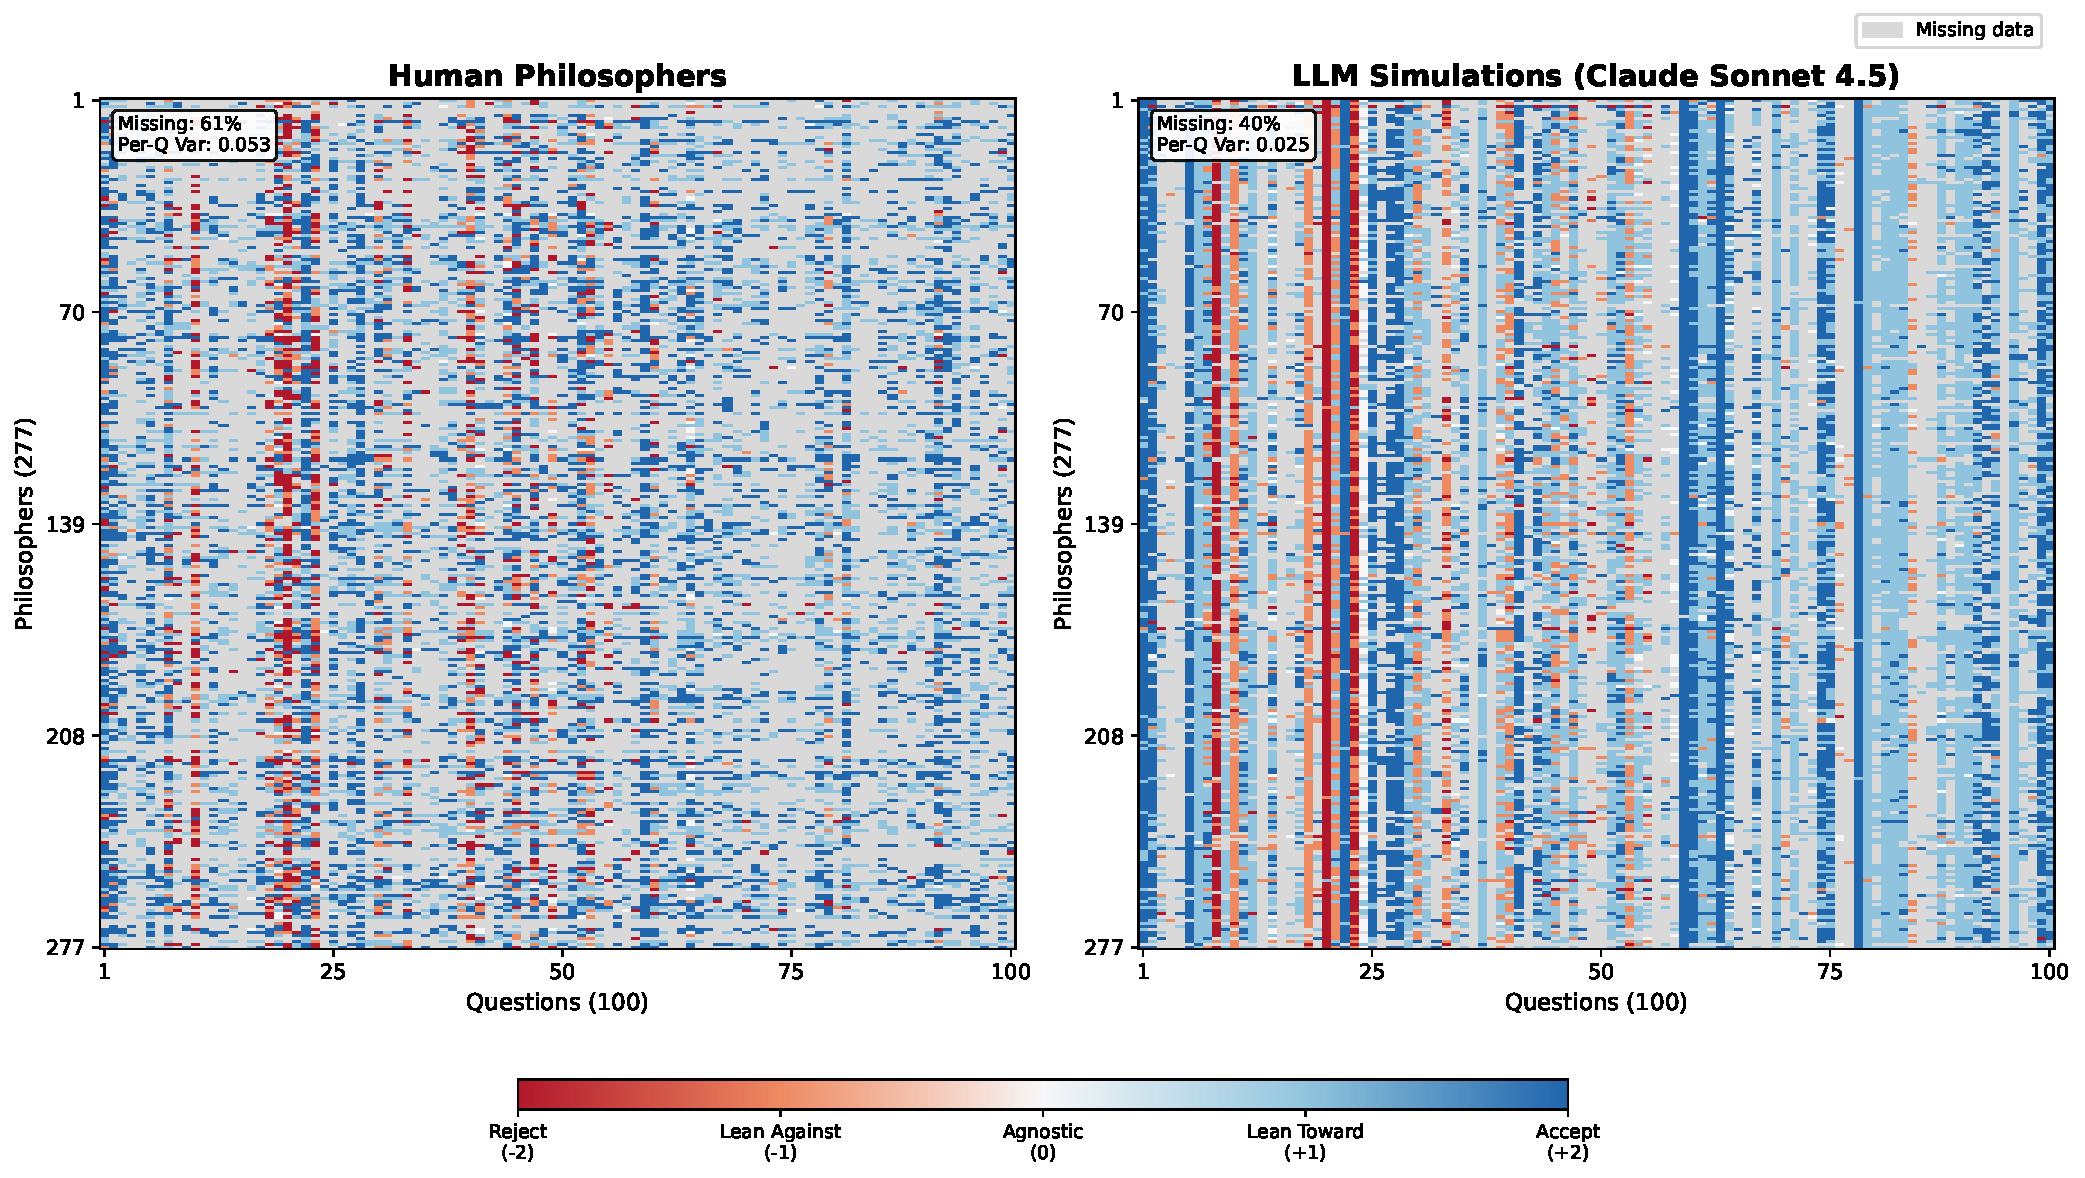
\includegraphics[width=\textwidth]{figures/figure1_human_vs_sonnet}
\end{center}

Each cell is one philosopher on one
question. Humans: Per-Q Var $=0.053$,
61\% missing. Claude: $0.025$, 40\%
missing.

\section{The induced world is flatter}
Across seven models, variance is
$1.4$--$2.4\times$ lower than humans.
Claude is uniform on 10 questions.

\section{And mis-shaped}
Human disagreement spans several
independent axes. Models cluster by
surface topic. DPO improves
correlations but does not restore
the distribution.

\section{Stereotypes fill the gap}
Where humans show no specialist
effect, models invent a large one:
\begin{itemize}
\item Biology $\to$ biological identity:
$+11$\,pp vs $+43$\,pp
\item Biology $\to$ psychological identity:
$+4$ vs $-66$\,pp
\item Ancient $\to$ Aristotelian reason:
$+2$ vs $+69$\,pp
\end{itemize}

}
\end{document}
